% ****** Start of file apssamp.tex ******
%
%   This file is part of the APS files in the REVTeX 4.1 distribution.
%   Version 4.1r of REVTeX, August 2010
%
%   Copyright (c) 2009, 2010 The American Physical Society.
%
%   See the REVTeX 4 README file for restrictions and more information.
%
% TeX'ing this file requires that you have AMS-LaTeX 2.0 installed
% as well as the rest of the prerequisites for REVTeX 4.1
%
% See the REVTeX 4 README file
% It also requires running BibTeX. The commands are as follows:
%
%  1)  latex apssamp.tex
%  2)  bibtex apssamp
%  3)  latex apssamp.tex
%  4)  latex apssamp.tex
%
\documentclass[%
 reprint,
%superscriptaddress,
%groupedaddress,
%unsortedaddress,
%runinaddress,
%frontmatterverbose,
%preprint,
%showpacs,preprintnumbers,
%nofootinbib,
%nobibnotes,
%bibnotes,
amsmath,amssymb,
%aps,
pra,
%prb,
%rmp,
%prstab,
%prstper,
%floatfix,
]{revtex4-1}

\usepackage{tabularx}
\usepackage{siunitx}
\sisetup{separate-uncertainty}
\usepackage{graphicx}% Include figure files
\usepackage{dcolumn}% Align table columns on decimal point
\usepackage{bm}% bold math
%\usepackage{hyperref}% add hypertext capabilities
%\usepackage[mathlines]{lineno}% Enable numbering of text and display math
%\linenumbers\relax % Commence numbering lines

%\usepackage[showframe,%Uncomment any one of the following lines to test
%%scale=0.7, marginratio={1:1, 2:3}, ignoreall,% default settings
%%text={7in,10in},centering,
%%margin=1.5in,
%%total={6.5in,8.75in}, top=1.2in, left=0.9in, includefoot,
%%height=10in,a5paper,hmargin={3cm,0.8in},
%]{geometry}

\begin{document}

\preprint{APS/123-QED}

\title{Atomic Force Microscopy}% Force line breaks with \\

\author{Moritz Berger}
 \altaffiliation[]{RWTH Aachen University, Germany}%Lines break automatically or can be forced with \\
 \email{moritz.berger@rwth-aachen.de}
 \author{Gerald Kolter}
 \altaffiliation[]{RWTH Aachen University, Germany}%Lines break automatically or can be forced with \\
 \email{gerald.kolter@rwth-aachen.de}

\date{July 4, 2019}
%\date{\yesterday} It is always \today, today,
             %  but any date may be explicitly specified

\begin{abstract}
Atomic force microscopy is a method used to make images of small structures, where  visual microscopy is not sufficient. However this method has several other advantages over other methods, especially because it allows the analysis of forces. In this paper the imaging process is analyzed for different modes and applications.
The force calibration constants were determined for different setups used in contact and tapping mode. The force calibration constant for the contact mode is several orders of magnitude smaller than the one for the tapping mode. The systematical error is dominating over the statistical. Furthermore a magnetic force analysis is carried out to determine the storage density of a hard drive. This density turns out to be significantly smaller than storage densities of modern hard drives.
\end{abstract}

\maketitle


\section{Introduction}
The Atomic Force Microscopy (AFM) gives an insight to the forces in a solid at atomic level. \\
An AFM consists of a sample holder, which is moved in x and y direction with a piezo crystal, and a tip mounted on a cantilever, which is moved in z direction (meaning the distance between tip and sample) with another piezo crystal. The bending of the cantilever with certain force constant is measured with a laser beam reflected on the flip side of the cantilever. \\
The AFM is used in three modes: Contact, Tapping and Magnetic Force. In contact mode the tip and sample are in contact. In tapping mode the tip is oscillating in a certain distance to the sample and tapping it which changes the amplitude of the oscillation and this gives the height of the sample at that point. Magnetic Force Microscopy (MFM) uses both the tapping mode and the fly mode, where the tip is kept at a constant distance away from the sample in order to measure long range forces. \\
The goal of the measurement is to determine the force constants of the cantilever in contact and tapping mode. With the MFM the goal is to analyze the magnetic structure of the sample. With that one can determine the possible storage density. \\
In section \ref{sec:Measurement} the measurement technique for all three modes is explained. The analysis of the data is explained in section \ref{sec:Data_Analysis} and the results are presented in section \ref{sec:Results}. In section \ref{sec:Conclusion} a conclusion for all analysis is made.


\section{Measurement}
\label{sec:Measurement}
\subsection{Contact Mode}
In contact mode the topology of a given sample is measured. In order to determine the optimal scan configuration an area is scanned for multiple different configurations. The optimal settings are listed in table \ref{tab:contact_settings}. With these settings the L-R, T-B and topology data of the sample is measured.\\
In a second part the force vs. distance curve (also referred to as snap-in curve) is measured. This is done by measuring the T-B data dependent on the distance. The cantilever starts in contact with the sample, is then moved \SI{800}{nm} away from the sample and then moved back to the original position.
\begin{table}[h]
\centering
\begin{tabular}{|c|c|c|c|c|}
\hline 
$K_i$ & $K_p$ & area & speed[lines/s] & setpoint\\ 
\hline 
20000 & 90000 & $\SI{5}{\mu m^2}$ & 2 & \SI{40}{mV}\\ 
\hline 
\end{tabular} 
\caption{Settings used for the contact mode.}
\label{tab:contact_settings}
\end{table}

\subsection{Tapping Mode}
In a first step the resonance frequency of the cantilever is determined by sweeping the frequency and measuring the amplitude, because knowledge of this frequency is necessary for the other measurements. The resonance frequency turns out to be \SI{263.8(1)}{kHz}, as seen in figure \ref{fig:res_tap}. In order to avoid full resonance a frequency of \SI{263.8}{kHz}, which is slightly off the resonance frequency, is used for the following measurements.\\
Next the amplitude, phase and topology of a different sample is measured in a similar process as the topology measurement in the contact mode. The optimal setting are given in table \ref{tab:tapping_settings}.\\
As a final measurement in this mode the cantilever amplitude is measured dependent on the distance between sample and tip in a similar procedure as the force-distance measurement in the contact mode. 
\begin{table}[h]
\centering
\begin{tabular}{|c|c|c|c|c|}
\hline 
$K_i$ & $K_p$ & area & speed[lines/s] & Frequency\\ 
\hline 
1800 & 5400 & $\SI{7}{\mu m^2}$ & 1.6 & \SI{263.8}{kHz}\\ 
\hline 
\end{tabular} 
\caption{Settings used for the tapping mode.}
\label{tab:tapping_settings}
\end{table}

\begin{figure}
\centering
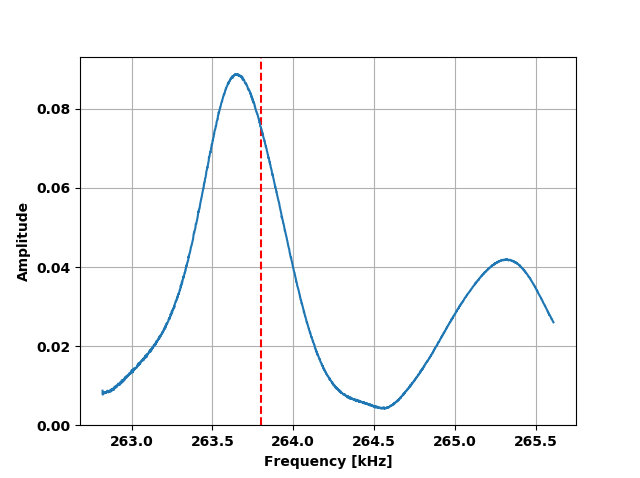
\includegraphics[scale=0.55]{Bilder/res_tapping}
\caption{Resonance spectrum of the tip used in tapping mode, zoomed into the largest peak. The red line indicates the frequency of \SI{263.8}{kHz} used for the measurements.}
\label{fig:res_tap}
\end{figure}

\subsection{Magnetic force microscopy}
Because the tapping mode is also used for parts of the magnetic measurement, the first step is again to determine the resonance frequency with the same method described for the tapping mode. Here the resonance frequency is \SI{76.09 \pm 0.06}{kHz} (as seen in figure \ref{fig:res_moag}) and a frequency of \SI{76.02}{kHz} is applied for the following measurements.\\
The second part is to determine the necessary Bias-Offset in order to be able to correct it. For this the Bias voltage is swept from \SI{-4}{V} to \SI{4}{V} and the amplitude and phase are measured.\\
Finally the magnetic domains of a hard drive are imaged. This is done by first scanning the amplitude and topology in tapping mode and then measuring the phase in fly mode. The settings used for this measurement are listed in table \ref{tab:magnetic_settings}. The measurement is done for 2 different area sizes in order to make the analysis of the domain dimensions easier.

\begin{table}[h]
\centering
\begin{tabular}{|c|c|c|c|c|c|c|}
\hline 
$K_i$ & $K_p$ & area & lines/s & Frequency & Bias & Scan height\\ 
\hline 
600 & 1800 & $\SI{20}{\mu m^2}$ & 1.6 & \SI{76.02}{kHz} & \SI{50}{mV} & \SI{25}{nm}\\ 
\hline 
1500 & 4500 & $\SI{30}{\mu m^2}$ & 1 & \SI{76.02}{kHz} & \SI{50}{mV} & \SI{25}{nm}\\ 
\hline 
\end{tabular} 
\caption{Settings used for the two measurements for the magnetic force microscopy.}
\label{tab:magnetic_settings}
\end{table}

\begin{figure}
\centering
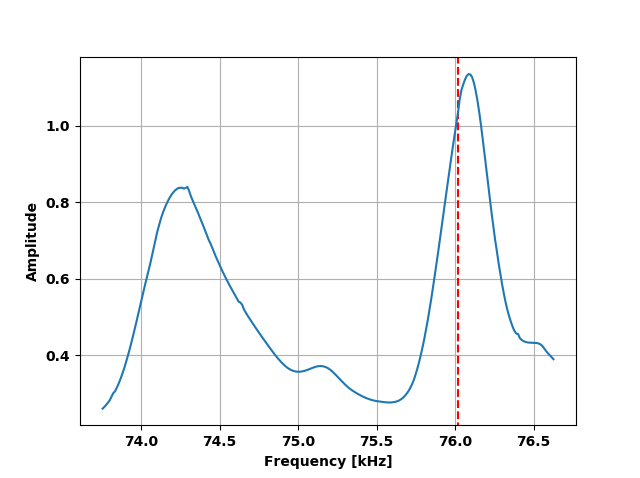
\includegraphics[scale=0.55]{Bilder/res_magnetic}
\caption{Resonance spectrum of the tip used in the magnetic mode, zoomed into the largest peak. The red line indicates the frequency of \SI{76.02}{kHz} used for the measurements.}
\label{fig:res_moag}
\end{figure}

\section{Data Analysis}
\label{sec:Data_Analysis}

\subsection{Contact and Tapping Mode}

\begin{table}[h]
\centering
\begin{tabular}{|c|c|c|}
\hline 
 & Contact Mode & Tapping Mode \\ 
\hline 
$k_{real}$ & (0.18 $_{+0.06} ^{-0.03}$) \si{N \per m} & (40 $_{+12} ^{-6}$) \si{N \per m} \\ 
\hline 
\end{tabular} 
\caption{Force constants of the cantilever as given by the producer.}
\label{tab:force_constants}
\end{table}

In both modes an area of a known sample is measured and a height profile is extracted to calculate the calibration constant. The height of the structures on all samples is given by:
\begin{equation*}
h_{real} = \SI{19 \pm 2}{nm}
\end{equation*}
For this purpose a height profile of a structure is extracted. At this profile there are five linear functions fitted: One on each flank, one in between the flanks and one on each side of the structure. The height is determined as the difference on the z-axes between the intersections of the linear fits. For this the difference is taken on the right and the left flank separatly and averaged afterwards. To get a good approximation and the error this is done multiple times. The calibration constant is calculated as:
\begin{equation*}
k_z = \dfrac{h_{real}}{h_{measured}}
\end{equation*}
For all modes the deflection is measured while approaching the sample with the tip from far away. After approaching the sample the tip is retracted again. In this measurement are linear regimes which follow the linear force-distance law. There are two linear regimes, one at the approaching and one at the retracting. At each there is a linear function fitted and the two slopes are averaged. With this one calculates the force-calibration constant as:
\begin{equation*}
k_F = \dfrac{k_{real} \cdot k_z}{\alpha}
\end{equation*}
In this $k_{real}$ denotes the known force constant of the cantilever (the force constants for the cantilever used in the different modes are listed in tab. \ref{tab:force_constants}), $k_z$ the calibration constant as given above and $\alpha$ is the averaged slope of the two fits mentioned above. \\

\section{Results}
\label{sec:Results}
\subsection{Contact Mode}

\begin{figure}[h]
\centering
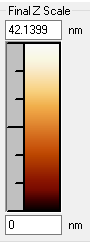
\includegraphics[scale=0.7]{Bilder/Contact_Mode/Rohdaten/try1_scalebar.PNG}
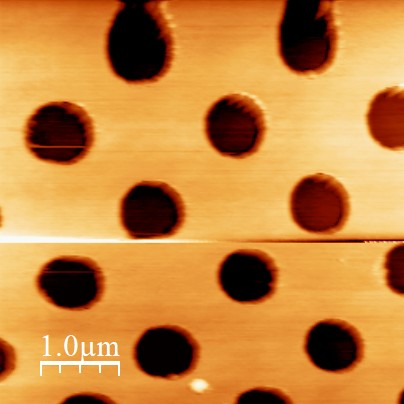
\includegraphics[scale=0.5]{Bilder/Contact_Mode/Rohdaten/try1.JPG}
\caption{Image from the sample recorded in contact mode.}
\label{fig:Contact_raw_data}
\end{figure}

\begin{table}[b]
\centering
\begin{tabular}{|c|c|c|}
\hline 
h$_1$ & h$_2$ & h$_3$ \\ 
\hline 
\SI{25.74 \pm 1.01}{nm} & \SI{25.88 \pm 1.01}{nm} & \SI{26.19 \pm 1.01}{nm} \\ 
\hline
h$_4$ & h$_5$ & h$_6$ \\ 
\hline 
\SI{26.00 \pm 1.01}{nm} & \SI{25.74 \pm 1.01}{nm} & \SI{23.13 \pm 1.01}{nm}  \\ 
\hline 
 h$_7$ & h$_8$ &  \\ 
\hline 
\SI{24.07\pm 1.01}{nm} & \SI{25.11 \pm 1.01}{nm} &  \\ 
\hline 
\end{tabular} 
\caption{Measured height for the structures in contact mode.}
\label{tab:Contact_height}
\end{table}

Fig. \ref{fig:Contact_raw_data} shows the measured image from the sample in contact mode. The height profiles are extracted from a straight line approximately through the center of the circles. \\
The measurement for the heights are listed in Tab. \ref{tab:Contact_height}. The height measurement therefor yield the following result:
\begin{equation*}
h_{measured}^{contact} = \SI{25.23 \pm 1.08}{nm}
\end{equation*}
With this the calibration constant can be calculated:
\begin{equation*}
k_z^{contact} = 0.75297 \pm 0.08560
\end{equation*}

\begin{figure}
\centering
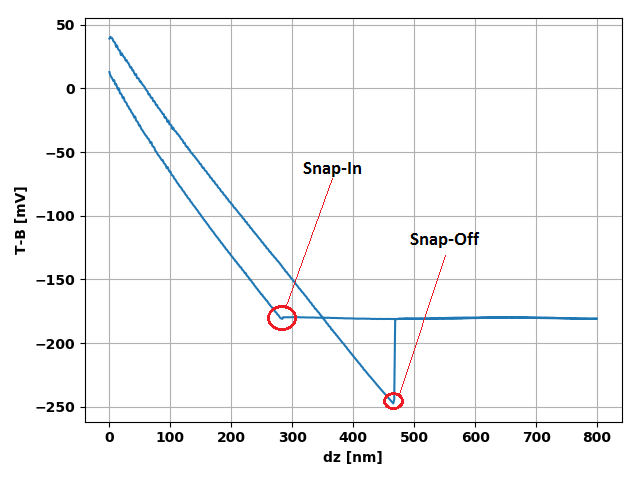
\includegraphics[scale=0.5]{Bilder/Contact_Mode/Snap_in_curve_marked.PNG}
\includegraphics[scale=0.5]{Bilder/Contact_Mode/Snap_in_curve_fit.PNG}
\caption{Snap-in curve measured in contact mode. The upper plot shows the measurement with marked snap-in and snap-off and the lower shows the fits to the linear regimes.}
\label{fig:Contact_snap_in}
\end{figure}

Fig. \ref{fig:Contact_snap_in} shows the snap-in curve measured with the setup used in the contact mode. The linear fit yields the averaged slope for the linear regime:
\begin{equation*}
|\alpha| = \SI{0.627 \pm 0.023}{V \per \mu m}
\end{equation*}
With this one calculates the force-calibration constant as:
\begin{equation*}
k_F^{contact} = (2.16 \pm 0.25 \, (stat.) \, _{+ 0.77} ^{- 0.42} \, (sys.)) \times 10^{-10} \si{N \per mV}
\end{equation*}

By determing the difference $\Delta _{adhesion}$ between the T-B Signal at the constant part and at the lowest point in the snap-in curve (fig. \ref{fig:Contact_snap_in}) one can calculate the adhesion force as:
\begin{equation*}
F_{adhesion} = \Delta _{adhesion} \cdot k_F^{contact}
\end{equation*}
The result is:
\begin{equation*}
F_{adhesion} = (1.43140 \pm 0.00023 \, (stat.) \, _{+ 0.50783} ^{- 0.28057} \, (sys.)) \times 10^{-8} \si{N}
\end{equation*}
The load force, meaning the force with which the tip is pressed onto the sample, can be calculated with the difference $\Delta _{load}$ between the T-B signal at the two points with $Z=0$ in the snap-in curve (fig. \ref{fig:Contact_snap_in}) as:
\begin{equation*}
F_{load} = \Delta _{load} \cdot k_F^{contact}
\end{equation*}
The result is:
\begin{equation*}
F_{load} = (5.68 \pm 0.19 \, (stat.) \, _{+ 2.01} ^{- 1.11} \, (sys.)) \times 10^{-9} \si{N}
\end{equation*}

\subsection{Tapping Mode}

\begin{figure}[h]
\centering
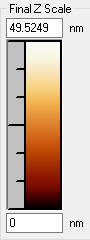
\includegraphics[scale=0.7]{Bilder/Tapping_Mode/Rohdaten/try3_scalebar.PNG}
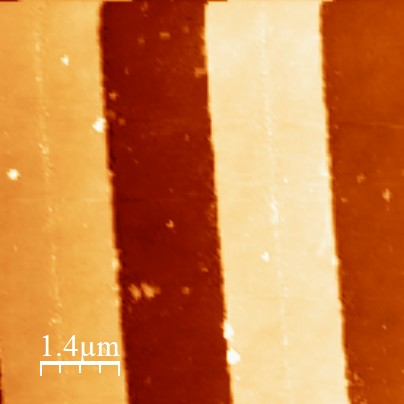
\includegraphics[scale=0.5]{Bilder/Tapping_Mode/Rohdaten/try3.JPG}
\caption{Image from the sample recorded in tapping mode.}
\label{fig:Tapping_raw_data}
\end{figure}

\begin{table}[b]
\centering
\begin{tabular}{|c|c|c|}
\hline 
h$_1$ & h$_2$ & h$_3$ \\ 
\hline 
\SI{27.13 \pm 0.39}{nm} & \SI{27.79 \pm 0.39}{nm} & \SI{26.90 \pm 0.39}{nm}  \\ 
\hline 
h$_4$ & h$_5$ & h$_6$ \\ 
\hline 
\SI{27.07 \pm 0.39}{nm} & \SI{27.09 \pm 0.39}{nm} & \SI{27.47 \pm 0.39}{nm}  \\ 
\hline 
 h$_7$ & & \\ 
\hline 
\SI{28.02 \pm 0.39}{nm} & &  \\ 
\hline 
\end{tabular} 
\caption{Measured height for the structures in tapping mode.}
\label{tab:Tapping_height}
\end{table}

Fig. \ref{fig:Tapping_raw_data} shows the mesured image from the sample in tapping mode. This looks different as in contact mode, because its an other area from an identical sample. The height profiles are extracted as straight lines perpendicular to the lines on the sample. \\
The measurement for the heights are listed in Tab. \ref{tab:Contact_height}. The height measurement therefor yield the following result:
\begin{equation*}
h_{measured}^{tapping} = \SI{27.35 \pm 0.42}{nm}
\end{equation*}
With this the calibration constant can be calculated:
\begin{equation*}
k_z^{tapping} = 0.695 \pm 0.074
\end{equation*}

\begin{figure}
\centering
%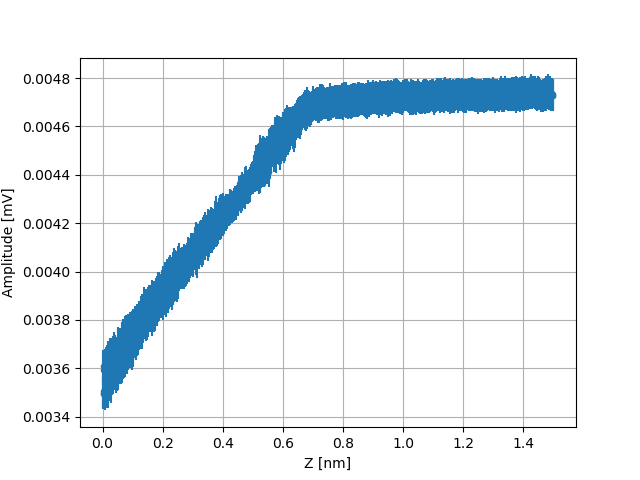
\includegraphics[scale=0.5]{Bilder/Tapping_Mode/Snap_in_curve.PNG}
\includegraphics[scale=0.5]{Bilder/Tapping_Mode/Snap_in_curve_fit.PNG}
\caption{Measured amplitude plotted against the sample-tip distance.}
\label{fig:Tapping_snap_in}
\end{figure}

Fig. \ref{fig:Tapping_snap_in} shows the measured amplitude plotted against the sample-tip distance with the setup used in the tapping mode. In the linear regime the oszillation amplitude decreases as the tip approaches the sample. This is due to the tip hitting the sample at its lower turning point. \\
The linear fit yields the averaged slope for the linear regime:
\begin{equation*} 
|\alpha| = \SI{1.6330 \pm 0.0057}{V \per \mu m}
\end{equation*}
With this one calculates the force-calibration constant as:
\begin{equation*}
k_F^{tapping} = (1.70 \pm 0.18 \, (stat.) \, _{+ 0.49} ^{- 0.25} \, (sys.)) \times 10^{-5} \si{N \per mV}
\end{equation*} 

The free oszillation amplitude is given by the plateau in fig. \ref{fig:Tapping_snap_in}. To determine the amplitude value of this plateau a linear fit to it is performed. As the slope of this fit matches with zero in a range of $2 \sigma$, one can use the y axis section as value for the plateau:
\begin{equation*}
b = \SI{4.686 \pm 0.019}{mV}
\end{equation*}
Given this value the free oszillation amplitude is determined by:
\begin{equation*}
\begin{aligned}
A_{free} = \dfrac{b}{\alpha}\\
A_{free} = \SI{2.87 \pm 0.10}{nm}
\end{aligned}
\end{equation*} \\

\begin{figure}
\centering
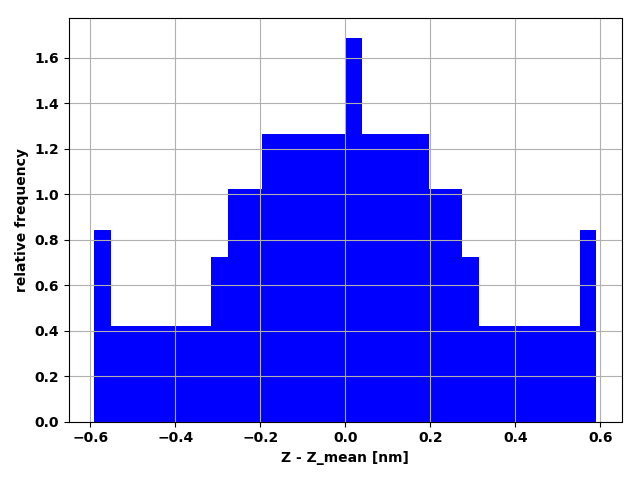
\includegraphics[scale=0.5]{Bilder/Tapping_Mode/Roughness_histogram.PNG}
\caption{Histogram of distances to the mean value of the plateau.}
\label{fig:Roughness_histogram}
\end{figure}

Fig. \ref{fig:Roughness_histogram} shows the histogram of the distance between measured points and the mean value of these. As expected the highest counts are around zero. The histogram shows a gaussian-shape. The diameter of a silicon atom is given by:
\begin{equation*}
d_{\text{silicon atom}} \approx \SI{111}{pm}
\end{equation*}
Given this value one can say that the roughness of the sample is in the order of a few atoms. \\
On the images made from the sample no clear contaminations can be found.


\subsection{Magnetic Microscopy}

\subsubsection{Contact Potential Difference}

\begin{figure}[h]
\centering
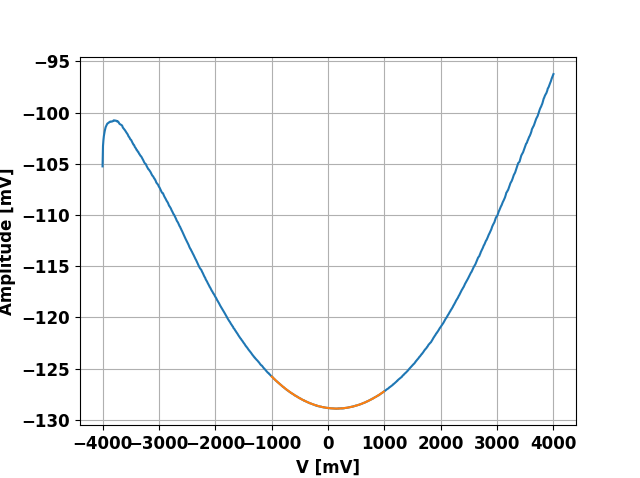
\includegraphics[scale=0.5]{Bilder/Magnetic/amplitude.PNG}
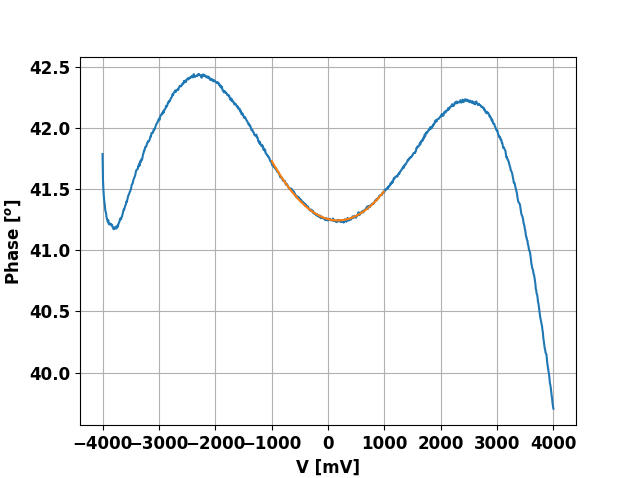
\includegraphics[scale=0.5]{Bilder/Magnetic/phase.PNG}
\caption{Amplitude (top) and Phase (bottom) plotted against the Bias-voltage. A parabolic function is fitted against the extemum in order to extract its offset from 0.}
\label{fig:bias}
\end{figure}

The contact potential difference is determined by varying the Bias voltage and recording the amplitude and phase. The Force experienced by the tip is proportional to
\begin{equation}
F \backsim \left(U-\dfrac{\Delta\Phi}{e}\right)^2
\end{equation}
where $U$ denotes the Bias-voltage and $\Delta\Phi$ the contact potential difference. As a consequence of this force both the amplitude and phase should experience a extremum at $\Delta\Phi / e$, which means one can simply extract $\Delta\Phi$ through:
\begin{equation}
\Delta\Phi = U_{extr} \cdot e
\label{eq:phi}
\end{equation}

For this a parabolic function is fitted against the data between \SI{-1}{V} and \SI{1}{V}, as seen in figure \ref{fig:bias}. The extremum and its error are directly extracted from this fit. It results in a position of
\begin{equation*}
U_{extr}^{amplitude} = \SI{151.7 \pm 0.3}{mV}
\end{equation*}
\begin{equation*}
U_{extr}^{phase} = \SI{174.8 \pm 1.6}{mV}
\end{equation*}
The weighted mean of the 2 values is
\begin{equation*}
U_{extr}^{mean} = \SI{152.5 \pm 4.2}{mV}
\end{equation*}
which is used to determine the final value of the contact potential difference with the help of equation \ref{eq:phi}:
\begin{equation*}
\Delta\Phi = \SI{152.5 \pm 4.2}{meV}
\end{equation*}

\subsubsection{Domain structure}
As a second part the domain structure of the sample is analyzed, as seen in figure \ref{fig:magnetic_domain}. There are three different areas with magnetic domains visible. Between these areas there is a small zone where no domains are visible.\\
In order to analyze the density of the domains the width of the areas is visually estimated. This is done by extracting 3 distances for each area alongside the visual structure from the beginning of one area to the beginning of the next, as shown in figure \ref{fig:magnetic_domain}. 
This is done for the \SI{20}{\mu m^2} scan as well as for the \SI{30}{\mu m^2} scan to increase accuracy and in order to verify that the measured areas have similar widths. The resulting average width of all 9 extracted values is
\begin{equation}
L = \SI{10.24 \pm 0.43}{\mu m}
\end{equation}
which is used for the density calculation.

\begin{figure}
\centering
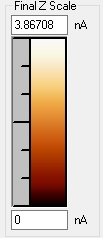
\includegraphics[scale=0.7]{Bilder/Magnetic/try2_scale.jpg}
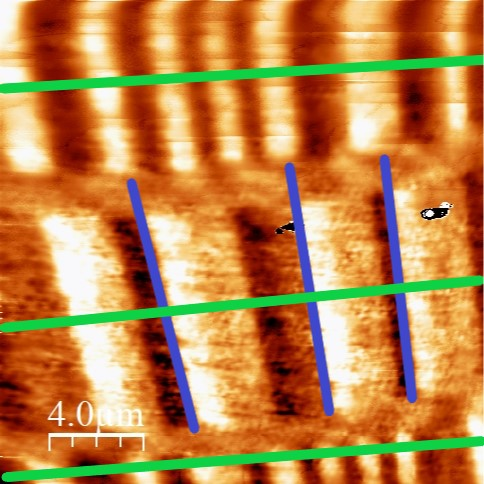
\includegraphics[scale=0.45]{Bilder/Magnetic/try2_lines.jpg}
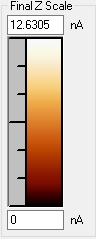
\includegraphics[scale=0.7]{Bilder/Magnetic/try4_scale.jpg}
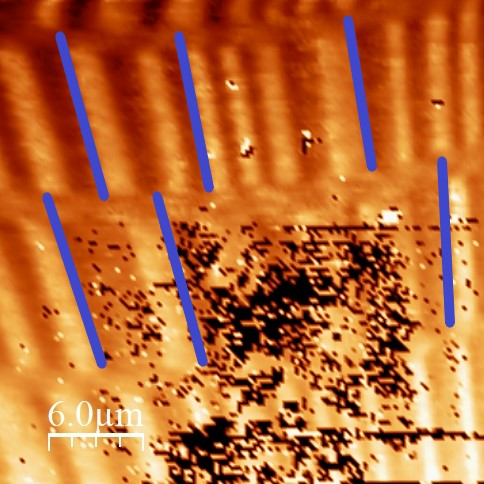
\includegraphics[scale=0.45]{Bilder/Magnetic/try4_lines.jpg}
\caption{Images of the phase in order to analyze the domain structure. The extracted distances for the width are marked by blue lines. The extracted height profiles are marked by green lines.}
\label{fig:magnetic_domain}
\end{figure}

Next a height profile of every area in the \SI{20}{\mu m^2} scan is extracted and the distance between the leftmost and rightmost peak measured. For this both the peak position and its error are visually estimated. The profile of the \SI{30}{\mu m^2} scan is not analyzed because there are a lot of points where the tip lost contact or crashed into the surface, which makes an analysis hard. The profiles can be found in figure \ref{fig:magnetic_profile}. The resulting peak distances are listed in table \ref{tab:magnetic_peaks}.

\begin{table}[h]
\centering
\begin{tabular}{|c|c|c|c|c|}
\hline 
area & left peak[$\mu m$] & right peak[$\mu m$] & distance[$\mu m$] & \#peaks/$\mu m^2$ \\ 
\hline 
top & $0.29 \pm 0.15$ & $18.64 \pm 0.05$ & $18.35 \pm 0.16$ & $0.032 \pm 0.001$\\ 
\hline
middle & $1.86 \pm 0.08$ & $16.91 \pm 0.28$ & $15.05 \pm 0.29$ & $0.019 \pm 0.001$\\ 
\hline
bottom & $1.65 \pm 0.16$ & $19.67 \pm 0.04$ & $18.02 \pm 0.16$ & $0.038 \pm 0.001$\\ 
\hline
\end{tabular} 
\caption{Peak positions and distance between them extracted from the height profiles. in order to calculate the \#peaks/$\mu m^2$ the number of peaks is divided by the distance and the average width L.}
\label{tab:magnetic_peaks}
\end{table}

\begin{figure}[h]
\centering
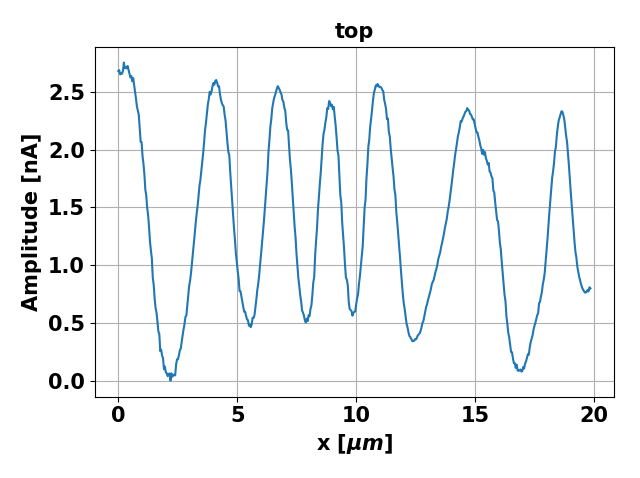
\includegraphics[scale=0.4]{Bilder/Magnetic/top.png}
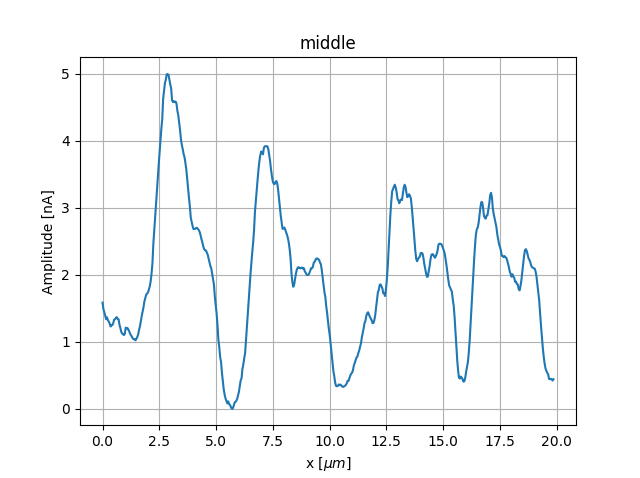
\includegraphics[scale=0.4]{Bilder/Magnetic/mid.png}
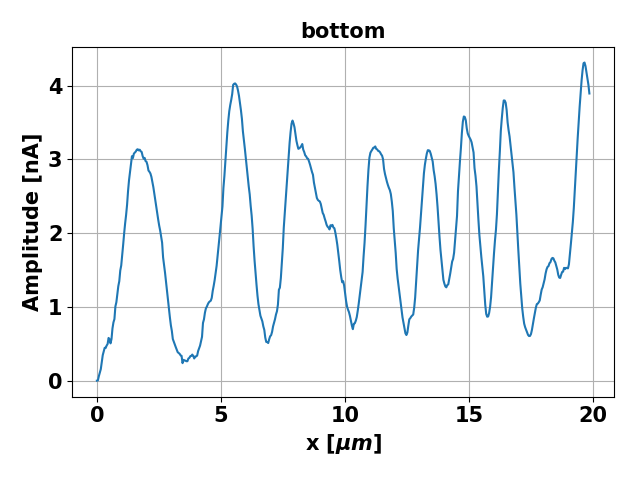
\includegraphics[scale=0.4]{Bilder/Magnetic/bot.png}
\caption{Extracted height profiles of the top, middle and bottom areas of the \SI{20}{\mu m^2} scan.}
\label{fig:magnetic_profile}
\end{figure}

In order to get an average density the results of the weighted average of the 3 areas is calculated:
\begin{equation*}
\#peaks/\mu m^2_{average} = 0.030 \pm 0.007
\end{equation*}
One peak equivalates to one domain, which saves exactly 1 Bit. This means that the storage density of the hard drive is
\begin{equation*}
\SI{19.3\pm 4.5}{MBit/in^2}
\end{equation*}

\section{Conclusion}
\label{sec:Conclusion}
$k_F^{contact}$ is several magnitudes of order smaller than $k_F^{tapping}$. As the voltage can be measured with the same certainty this means that in contact mode the resolution with which the the force on the cantilever can be measured is much higher than in tapping mode. This makes sense as the forces to be measured in cantact mode are smaller than those in tapping mode. \\
The statistical error on the force calibration constants is about 10\%. The systematical error only due to the error on the known force constant of the cantilever is with up to 35\% much higher. 
\\
The storage density of the analyzed hard drive is \SI{19.3\pm 4.5}{MBit/in^2}. However the density varies nearly by a factor 2 depending on which area of the image is analyzed. This makes it possible that there is a big systematical error in this result, and a bigger area with more Bits is needed to give an accurate estimation of the storage density.\\
Modern hard drives can reach a storage density of \SI{5}{GBit/in^2} - \SI{20}{GBit/in^2} \cite{Loss98}, which is a factor 1000 bigger than the result of this analysis.







\bibliography{AFM}% Produces the bibliography via BibTeX.

\end{document}
